\documentclass[a4paper]{article}

\usepackage{amsmath}
\usepackage{amssymb}
\usepackage{amsfonts}
\usepackage[style=iso]{datetime2}
\usepackage[explicit]{titlesec}
\usepackage{amsthm}
\usepackage{mathrsfs}
\usepackage{array}
\usepackage{graphicx}
\usepackage{mathtools} % Provides \mathrlap command
\usepackage{float}
\usepackage[skip=1em,indent]{parskip}
\usepackage{caption}
\usepackage[hidelinks]{hyperref}
\usepackage{tocloft}
\usepackage{mathtools}
\usepackage{enumitem}

\usepackage{tikz}
\tikzset{>=latex} % for LaTeX arrow head
\usepackage{pgfplots} % for the axis environment
\usetikzlibrary{calc,decorations.markings}

\pgfplotsset{compat=1.18, every tick label/.append style={font=\footnotesize}}

\graphicspath{ {./Images/} }

\makeatletter
\def\th@plain{%
  \thm@notefont{}% same as heading font
  \itshape % body font
}
\def\th@definition{%
  \thm@notefont{}% same as heading font
  \normalfont % body font
}
\makeatother

\newcommand*\diff{\mathop{}\!d} % for the differential in integrals

% ---------------- %
\newcommand{\R}{\mathbb{R}}
\newcommand{\C}{\mathbb{C}}
\newcommand{\Z}{\mathbb{Z}}

\NewCommandCopy{\oldIm}{\Im}
\renewcommand{\Im}{\mathop{\oldIm\mathfrak{m}}}
\NewCommandCopy{\oldRe}{\Re}
\renewcommand{\Re}{\mathop{\oldRe\mathfrak{e}}}

\newcommand{\overbar}[1]{\mkern 1.5mu\overline{\mkern-1.5mu#1\mkern-1.5mu}\mkern 1.5mu}

\DeclareMathOperator{\Res}{Res}
% ---------------- %

\newtheorem{theorem}{Theorem}
\newtheorem{lemma}[theorem]{Lemma}
\newtheorem{proposition}[theorem]{Proposition}
\newtheorem{corollary}{Corollary}[theorem]

\theoremstyle{definition}
\newtheorem{definition}[theorem]{Definition}
\newtheorem{example}[theorem]{Example}

% \setlength{\cftsecnumwidth}{3em}

\begin{titlepage}
\title{The Mellin Transform}
\author{Abdul Musthakin}
\date{July 2025}
\end{titlepage}

% \renewcommand{\thesection}{\Roman{section}}

\allowdisplaybreaks

\setlength{\parindent}{0pt}

\begin{document}
\maketitle

The \emph{Mellin transform} is an integral transform, similar to the \emph{Laplace transform} and the \emph{Fourier transform}.
Whilst it has many applications in mathematics, physics, and engineering, we will focus on proving a particular theorem related to the transform: \emph{Ramanujan's master theorem}.
\begin{definition}[Mellin Transform]
    Let $f \colon \R_{>0} \to \C$ be a function of $t$.
    The \emph{Mellin transform} of $f$, denoted $\mathcal{M}\{f\}$, is a function of $s \in \C$ defined by
    \begin{equation}
        \mathcal{M}\{f\}(s) \coloneq \int_0^\infty f(t) t^{s-1} \diff t,
    \end{equation}
    wherever this integral converges.
\end{definition}
\begin{definition}[Fundamental Strip]
    Let $\alpha, \beta \in \overline{\R}$, and let the open strip $\langle \alpha, \beta\rangle$ be defined for all $s \in \C$ such that $s \coloneq \sigma + it$ and $\alpha < \sigma < \beta$.
    The \emph{fundamental strip} of $\mathcal{M} \{f\}(s)$ is the largest open strip on which it is defined.
\end{definition}
We can evaluate the Mellin transform of various functions and determine their corresponding fundamental strips.
\begin{example}
    Let the function $f \colon \R_{>0} \to \C$ be defined by $f(t) \coloneq e^{-t}$.
    The Mellin transform of $f$ is then given by
    \begin{equation*}
        \mathcal{M}\left\{e^{-t}\right\} = \int_0^\infty e^{-t} t^{s-1} \diff t \eqcolon \Gamma(s),
    \end{equation*}
    where $\Gamma$ is the gamma function.
    As $\Gamma(s)$ is analytic for $\Re s > 0$, the fundamental strip is $\langle 0, +\infty \rangle$.
\end{example}
\begin{example}
    Let the function $f \colon \R_{>0} \to \C$ be defined by
    \begin{equation*}
        f(t) \coloneq \frac{1}{1+t}.
    \end{equation*}
    The Mellin transform of $f$ is given by
    \begin{equation*}
        \mathcal{M}\{f(t)\}(s) = \int_0^\infty \frac{t^{s-1}}{1+t} \diff t.
    \end{equation*}
    First, we wish to show that this integral converges and under what conditions that happens.
    \begin{proposition} \label{thm:mellin converge}
        The integral
        \begin{equation*}
            \mathcal{M}\{f(t)\}(s) = \int_0^\infty \frac{t^{s-1}}{1+t} \diff t
        \end{equation*}
        converges if and only if $0 < \Re s < 1$.
    \end{proposition}
    \begin{proof}
        Let $\sigma \coloneq \Re s$ and $\tau \coloneq \Im s$ giving us $s = \sigma + \tau i$.
        We can rewrite our integral and split it as follows.
        \begin{align*}
            \int_0^\infty \frac{t^{s-1}}{1+t} \diff t & = \int_0^\infty \frac{t^{\sigma-1+\tau i}}{1+t} \diff t                                                                                                                                      \\
                                                      & = \int_0^\infty \frac{t^{\sigma-1} t^{\tau i}}{1+t} \diff t                                                                                                                                  \\
                                                      & = \int_0^\infty \frac{t^{\sigma-1} e^{\tau i \ln t}}{1+t} \diff t                                                                                                                            \\
                                                      & = \underbrace{\int_0^\infty \frac{t^{\sigma-1} \cos(\tau \ln t)}{1+t} \diff t}_{\mathcal{I}} + i \underbrace{\int_0^\infty \frac{t^{\sigma-1} \sin(\tau \ln t)}{1+t} \diff t}_{\mathcal{J}}.
        \end{align*}
        Note that $\mathcal{M}\{f(t)\}(s)$ will converge if and only if both $\mathcal{I}$ and $\mathcal{J}$ converge.
        Consider $\mathcal{I}$ and split it into two integrals.
        \begin{equation*}
            \int_0^\infty \frac{t^{\sigma-1} \cos(\tau \ln t)}{1+t} \diff t = \underbrace{\int_0^1 \frac{t^{\sigma-1} \cos(\tau \ln t)}{1+t} \diff t}_{\mathcal{I}_1} + \underbrace{\int_1^\infty \frac{t^{\sigma-1} \cos(\tau \ln t)}{1+t} \diff t}_{\mathcal{I}_2}
        \end{equation*}
        Again, $\mathcal{I}$ will converge if and only if both $\mathcal{I}_1$ and $\mathcal{I}_2$ converge.
        For the integral from 0 to 1, the integrand is continuous everywhere on the interval except at $t=0$.
        We can bound the integral above as follows.
        \begin{alignat*}{3}
            \int_0^1 \frac{t^{\sigma-1} \cos(\tau \ln t)}{1+t} \diff t & \leq \int_0^1 \left\lvert \frac{t^{\sigma-1} \cos(\tau \ln t)}{1+t} \right\rvert \diff t \quad &  &                                                         \\
                                                                       & \leq \int_0^1 \frac{t^{\sigma-1}}{1+t} \diff t \qquad                                          &  & \because \cos x \leq 1                                  \\
                                                                       & \leq \int_0^1 t^{\sigma-1} \diff t \qquad                                                      &  & \because \frac{1}{1+t} \leq 1 \text{ for } t \in [0,1].
        \end{alignat*}
        Since $\sigma>0$, the last integral converges, so $\mathcal{I}_1$ converges as well.
        For the $\mathcal{I}_2$, first note that
        \begin{equation*}
            1+t \geq t \implies \frac{1}{1+t} \leq \frac{1}{t} \implies \frac{t^{\sigma-1}}{1+t} \leq t^{\sigma-2}.
        \end{equation*}
        Using this, we get
        \begin{equation*}
            \int_1^\infty \frac{t^{\sigma-1} \cos(\tau \ln t)}{1+t} \diff t \leq \int_1^\infty \frac{t^{\sigma-1}}{1+t} \diff t \leq \int_1^\infty t^{\sigma-2} \diff t.
        \end{equation*}
        Since $\sigma < 1$, the last integral converges, so $\mathcal{I}_2$ converges as well.
        It thus follows that $\mathcal{I}$ converges.
        It can similarly be shown that $\mathcal{J}$ converges.
        Therefore, if $0 < \sigma < 1$, then
        \begin{equation*}
            \mathcal{M}\{f(t)\}(s) = \int_0^\infty \frac{t^{s-1}}{1+t} \diff t
        \end{equation*}
        converges.

        We now wish to show the converse.
        As the contrapositive of the converse -- `if $\sigma \leq 0$ or $\sigma \geq 1$, then the integral diverges' -- is equivalent to the converse itself (and easier to work with), we will prove that instead.
        First, consider the case where $s \in \R$; note that the integrand is positive.
        If $s = \sigma \geq 1$, then
        \begin{equation*}
            \int_1^\infty \frac{t^{s-1}}{1+t} \diff t \geq \int_1^\infty \frac{\diff t}{1+t}.
        \end{equation*}
        If $s = \sigma \leq 0$, then
        \begin{equation*}
            \int_0^1 \frac{t^{s-1}}{1+t} \diff t \geq \int_0^1 \frac{\diff t}{t(1+t)} \geq \int_0^1 \frac{\diff t}{2t}
        \end{equation*}
        Either way, for $s \in \R$, a part of $\mathcal{M}\{f(t)\}(s)$ is bounded below by a divergent integral, so $\mathcal{M}\{f(t)\}(s)$ diverges.
        Otherwise, consider $s \notin \R$, meaning that $\tau \neq 0$.
        Without loss of generality, assume that $\tau > 0$.
        Consider $\mathcal{J}$ under the substitution $t = e^x$.
        \begin{align*}
            \int_0^\infty \frac{t^{\sigma-1} \sin(\tau \ln t)}{1+t} \diff t & = \int_{-\infty}^\infty \frac{e^{(\sigma-1)x}\sin(\tau x)}{1+e^x} \cdot e^x \diff x \\
                                                                            & = \int_{-\infty}^\infty \frac{e^{\sigma x}\sin(\tau x)}{1+e^x} \diff x
        \end{align*}
        Let
        \begin{equation*}
            \mathcal{J}_k \coloneq \int_{a_k}^{b_k} \frac{e^{\sigma x}\sin(\tau x)}{1+e^x} \diff x,
        \end{equation*}
        where $k \in \Z_{>0}$,
        \begin{equation*}
            a_k \coloneq \frac{2\pi k}{\tau},
        \end{equation*}
        and
        \begin{equation*}
            b_k \coloneq \frac{\pi(2k+1)}{\tau}.
        \end{equation*}
        If $\sigma \geq 1$, for $x \geq 0$, we have
        \begin{equation*}
            \frac{e^{\sigma x}}{1+e^x} \geq \frac{e^x}{1+e^x} \geq \frac{1}{2}.
        \end{equation*}
        As $\mathcal{J}_k \geq 0$ for all $k$,
        \begin{equation*}
            \int_{a_k}^{b_k} \frac{e^{\sigma x}\sin(\tau x)}{1+e^x} \diff x \geq \frac{1}{2} \int_{a_k}^{b_k} \sin(\tau x) \diff x = \frac{1}{\tau}.
        \end{equation*}
        If
        \begin{equation*}
            \int_{-\infty}^\infty \frac{e^{\sigma x}\sin(\tau x)}{1+e^x} \diff x,
        \end{equation*}
        converges, then
        \begin{equation*}
            \lim_{R \to \infty} \int_{-\infty}^R \frac{e^{\sigma x}\sin(\tau x)}{1+e^x} \diff x
        \end{equation*}
        exists, which would be true only if there exists some $x_0 \in \R$ such that
        \begin{equation*}
            \left\lvert \int_{-\infty}^{R_1} \frac{e^{\sigma x}\sin(\tau x)}{1+e^x} \diff x - \int_{-\infty}^{R_2} \frac{e^{\sigma x}\sin(\tau x)}{1+e^x} \diff x \right\rvert < \frac{1}{2\tau}
        \end{equation*}
        for all $R_1, R_2 \geq x_0$.
        Assume, for the purpose of contradiction, that such an $x_0$ exists.
        As $\ln a_k \to \infty$ and $\ln b_k \to \infty$, there exists some $k$ such that $\ln b_k > \ln a_k > x_0$, and
        \begin{align*}
            \left\lvert \int_{-\infty}^{b_k} \frac{e^{\sigma x}\sin(\tau x)}{1+e^x} \diff x - \int_{-\infty}^{a_k} \frac{e^{\sigma x}\sin(\tau x)}{1+e^x} \diff x \right\rvert & = \left\lvert \int_{a_k}^{b_k} \frac{e^{\sigma x}\sin(\tau x)}{1+e^x} \diff x \right\rvert \\
                                                                                                                                                                               & \geq \frac{1}{\tau}                                                                        \\
                                                                                                                                                                               & > \frac{1}{2\tau}.
        \end{align*}
        This is a contradiction, so there cannot exist such an $x_0$.
        Thus, if $\sigma \geq 1$,
        \begin{equation*}
            \int_{-\infty}^\infty \frac{e^{\sigma x}\sin(\tau x)}{1+e^x} \diff x
        \end{equation*}
        diverges if, meaning that $\mathcal{J}$ diverges as well.
        Therefore, if $\sigma \geq 1$,
        \begin{equation*}
            \mathcal{M}\{f(t)\}(s) = \int_0^\infty \frac{t^{s-1}}{1+t} \diff t.
        \end{equation*}
        diverges.
        A similar argument works to show that it diverges if $\sigma \leq 0$; we would consider negative $k$.
        Hence, if $\sigma \leq 0$ or $\sigma \geq 1$, the intergral diverges -- and the contrapositive of the statement is true as well.
        That finally completes the proof that the integral converges if and only if $0 < \sigma < 1$.
    \end{proof}
    There are various ways to evaluate this improper integral.
    One way is via contour integration.
    Consider
    \begin{equation*}
        \frac{z^{s-1}}{1+z}
    \end{equation*}
    for $z \in \C$.
    The numerator can be rewritten as $e^{(s-1) \log z}$ term, which is multivalued if $s \notin \Z$; we need to choose a branch of the logarithm.
    Choose the branch such that the argument of the logarithm ranges from 0 to $2\pi$, and let the branch cut be at the positive real axis.
    That is, given $z \coloneq e^{i \theta}$, we have $\log z \coloneq \ln \lvert z \rvert + i\theta$, where $0 \leq \theta < 2\pi$.
    Let the function $g \colon \C \setminus \{0, -1\} \to \C$ defined by
    \begin{equation*}
        g(z) \coloneq \frac{z^{s-1}}{1+z},
    \end{equation*}
    with the branch that we have chosen.
    This function has a simple pole at $(-1,0)$.
    The residue of the pole is given by
    \begin{align*}
        \Res (g,-1) & = \lim_{z \to -1} (z-(-1))g(z) \\&= \lim_{z \to -1} \frac{z^s}{z} \\&= -(-1)^s \\&= -e^{\pi i s}.
    \end{align*}
    There is also a singularity at the origin, as long as $s \notin \Z_{\geq 1}$.
    If $s \in \Z_{<1}$, then the singularity is a pole of order $1-s$ whose resiude is given by
    \begin{align*}
        \Res (g, 0) & = \frac{1}{(-s)!} \lim_{z \to 0} \frac{d^{-s}}{dz^{-s}} \left[ (z-0)^{1-s} g(z) \right]                                   \\
                    & = \frac{1}{\lvert s \rvert!} \lim_{z \to 0} \frac{d^{\lvert s \rvert}}{dz^{\lvert s \rvert}} \left[ \frac{1}{1+z} \right] \\
                    & = \frac{1}{\lvert s \rvert!} \lim_{z \to 0} \frac{(-1)^s}{(1+z)^{1-s}}                                                    \\
                    & = \frac{(-1)^s}{\lvert s \rvert!}
    \end{align*}
    Otherwise, the singularity is a branch point.
    Both singularities, as well as the possible branch cut, are shown in Figure~\ref{fig:contour}.

    Let $l_1$ and $l_2$ be horizontal lines from $(R,\delta)$ to $(\varepsilon, \delta)$ and $(R, -\delta)$ to $(\varepsilon, -\delta)$ respectively.
    Then, let $\Gamma$ be the circular arc going from $(R,\delta)$ to $(R, -\delta)$ and let $\gamma$ be the circular arc going from $(\epsilon, -\delta)$ to $(\varepsilon, \delta)$.
    Consider the contour $C$ defined by $C \coloneq \Gamma \cup l_2 \cup \gamma \cup l_1$.
    This is a positvely-oriented circular keyhole contour, as shown in Figure~\ref{fig:contour}.
    \begin{figure}[H]
        \centering
        \scalebox{1.39}{
            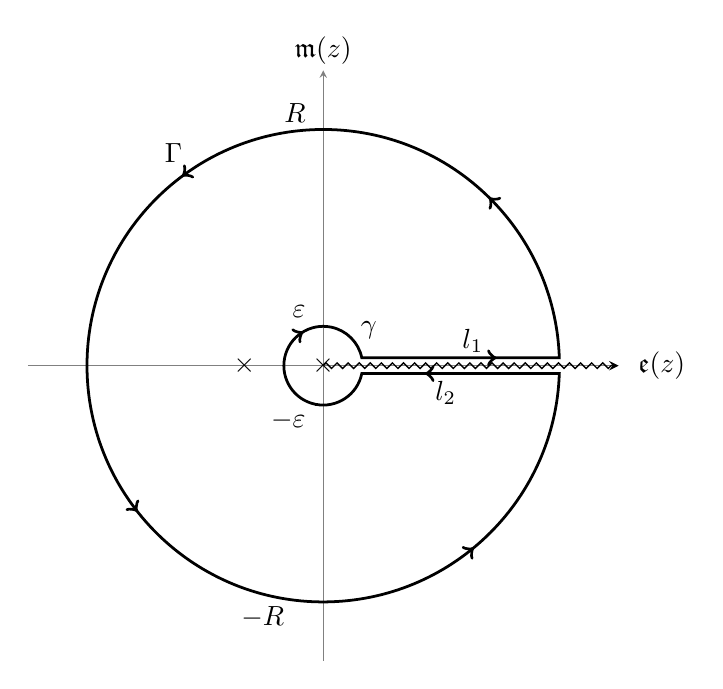
\begin{tikzpicture}
                % Configurable parameters
                \def\gap{0.2}
                \def\bigradius{3}
                \def\littleradius{0.5}

                % Axes
                \draw [help lines,-stealth] (-1.25*\bigradius, 0) -- (1.25*\bigradius,0);
                \draw [help lines,-stealth] (0, -1.25*\bigradius) -- (0, 1.25*\bigradius);
                \draw [decorate, decoration={zigzag, segment length=4, amplitude=1, post=lineto, post length=2}, line width=0.5pt, -stealth] (0,0) -- (1.25*\bigradius,0); % Zig-zag branch cut on the positive real axis
                % Red path
                \draw[line width=1pt,   decoration={ markings,
                            mark=at position 0.0855 with {\arrow[line width=1.2pt]{to}},
                            mark=at position 0.2455 with {\arrow[line width=1.2pt]{to}},
                            mark=at position 0.4255 with {\arrow[line width=1.2pt]{to}},
                            mark=at position 0.6055 with {\arrow[line width=1.2pt]{to}},
                            mark=at position 0.765 with {\arrow[line width=1.2pt]{to}},
                            mark=at position 0.87 with {\arrow[line width=1.2pt]{to}},
                            mark=at position 0.97 with {\arrow[line width=1.2pt]{to}}},
                    postaction={decorate}]
                let
                \n1 = {asin(\gap/2/\bigradius)},
                \n2 = {asin(\gap/2/\littleradius)}
                in (\n1:\bigradius) arc (\n1:360-\n1:\bigradius)
                -- (-\n2:\littleradius) arc (-\n2:-360+\n2:\littleradius)
                -- cycle;

                % The labels
                \node at (4.3,0){$\Re(z)$};
                \node at (0,4) {$\Im(z)$};
                \node at (0.58,0.45) {$\gamma$};
                \node at (-1.9,2.7) {$\Gamma$};
                \node at (1.9,0.32) {$l_1$};
                \node at (1.555,-0.35) {$l_2$};

                % The poles
                \node at (0,0) {$\times$};
                \node at (-1, 0) {$\times$};

                % Marks on the imaginary axis
                \draw (0,-\bigradius) -- ++(-0.1,0) node[left, yshift=-0.2cm] {$-R\phantom{-}$}; % Shift -R upward
                \draw (0,-\littleradius) -- ++(-0.1,0) node[left, yshift=-0.2cm] {$-\varepsilon$}; % Shift -ε upward
                \draw (0,\littleradius) -- ++(-0.1,0) node[left, yshift=0.2cm] {$\vphantom{-}\varepsilon$}; % Shift ε upward
                \draw (0,\bigradius) -- ++(-0.1,0) node[left, yshift=0.2cm] {$\vphantom{-}R$}; % Shift R upward

            \end{tikzpicture}}
        \captionsetup{justification=centering}
        \caption{The complex contour $C$}
        \label{fig:contour}
    \end{figure}
    By the \emph{residue theorem}, the contour integral along $C$ is given by
    \begin{equation*}
        \oint_C g(z) \diff z = 2 \pi i \Res (g, -1) = - 2 \pi i e^{\pi i s}
    \end{equation*}
    We can also consider the contour integral along $C$ as the integrals along the four parts of $C$.
    \begin{equation*}
        \oint_C g(z) \diff z = \int_\Gamma g(z) \diff z + \int_\gamma g(z) \diff z + \int_{l_1} g(z) \diff z + \int_{l_2} g(z) \diff z
    \end{equation*}
    The integral along $l_1$ can be evaluated via the parameterisation $z(t) \coloneq t + \delta i$ for $t \in [\varepsilon, R]$.
    \begin{align*}
        \int_{l_1} g(z) \diff z \coloneq & \int_{l_1} \frac{z^{1-s}}{1+z} \diff z                             \\
        \coloneq                         & \int_\varepsilon^R \frac{(z(t))^{s-1}}{1+z(t)} \cdot z'(t) \diff t \\
        =                                & \int_\varepsilon^R \frac{(t+\delta i)^{s-1}}{1+t+\delta i} \diff t
    \end{align*}
    We only care about this in the limit as $\delta$ approaches $0^+$.
    \begin{proposition} \label{thm:delta dct}
        \begin{equation*}
            \lim_{\delta \to 0^+} \int_\varepsilon^R \frac{(t+\delta i)^{s-1}}{1+t+\delta i} \diff t = \int_\varepsilon^R \lim_{\delta \to 0^+} \frac{(t+\delta i)^{s-1}}{1+t+\delta i} \diff t
        \end{equation*}
    \end{proposition}
    \begin{proof}
        Let $(w_{\delta_n})$ be the sequence of functions where
        \begin{equation*}
            w_{\delta_n} \coloneq \frac{(t+\delta_n i)^{s-1}}{1+t+\delta_n i}
        \end{equation*}
        for $t \in [\varepsilon, R]$, and $(\delta_n) \to 0^+$ is arbitrary.
        Since $t > 0$, we have $t+\delta_n i \to t$ and $\arg(t+\delta_n i) \to 0$ as $n \to \infty$.
        Thus,
        \begin{equation*}
            \lim_{\delta \to 0^+} w_{\delta_n} = \lim_{n \to \infty} w_{\delta_n} = \frac{t^{s-1}}{1+t}
        \end{equation*}
        pointwise for $t \in [\varepsilon, R]$.
        Now, we wish to show that the sequence is dominated by an integrable function.
        Let $\sigma \coloneq \Re s$ and $\tau \coloneq \Im s$.
        Then,
        \begin{align*}
            \left\lvert (t + \delta_n i)^{s-1} \right\rvert & = \left\lvert (t + \delta_n i)^{\sigma-1+\tau i} \right\rvert                                                                                                                                                                                                      \\
                                                            & = \left\lvert e^{(\sigma-1+\tau i)\log(t + \delta_n i)} \right\rvert                                                                                                                                                                                               \\
                                                            & = \left\lvert e^{(\sigma-1+\tau i)(\ln\lvert t + \delta_n i\rvert + i \arg(t + \delta_n i))} \right\rvert                                                                                                                                                          \\
                                                            & = \left\lvert e^{(\sigma-1) \ln\lvert t + \delta_n i\rvert} \right\rvert \left\lvert e^{(\sigma-1) i \arg(t + \delta_n i)} \right\rvert \left\lvert e^{\tau i \ln\lvert t + \delta_n i\rvert} \right\rvert \left\lvert e^{- \tau \arg (t+\delta_n i)} \right\rvert \\
                                                            & = \left\lvert e^{(\sigma-1) \ln\lvert t + \delta_n i\rvert} \right\rvert \left\lvert e^{- \tau \arg (t+\delta_n i)} \right\rvert                                                                                                                                   \\
                                                            & = \lvert t + \delta_n i \rvert^{\sigma-1} \cdot e^{- \tau \arg (t+\delta_n i)}.
        \end{align*}
        Due to the branch of the logarithm we have chosen, $\arg(t+\delta_n i) \in [0, 2\pi)$.
        Thus,
        \begin{align*}
            \left\lvert (t + \delta_n i)^{s-1} \right\rvert & = \lvert t + \delta_n i \rvert^{\sigma-1} \cdot e^{- \tau \arg (t+\delta_n i)} \\
                                                            & \leq \lvert t + \delta_n i \rvert^{\sigma-1} \cdot e^{-\tau \cdot 0}           \\
                                                            & = \lvert t + \delta_n i \rvert^{\sigma-1}
        \end{align*}
        if $\tau \geq 0$, and
        \begin{align*}
            \left\lvert (t + \delta_n i)^{s-1} \right\rvert & = \lvert t + \delta_n i \rvert^{\sigma-1} \cdot e^{- \tau \arg (t+\delta_n i)}   \\
                                                            & \leq \lvert t + \delta_n i \rvert^{\sigma-1} \cdot e^{-\tau \cdot \frac{\pi}{2}}
        \end{align*}
        if $\tau < 0$.
        This bound is independent of $\delta_n$ and $t$.
        Additionally, as $t \geq \varepsilon > 0$,
        \begin{equation*}
            \lvert 1 + t + \delta_n i \rvert = \sqrt{(1+t)^2 + \delta_n^2} \geq 1 + t \implies \frac{1}{\lvert 1 + t + \delta_n i \rvert} \leq \frac{1}{1+t}.
        \end{equation*}
        Since $\sigma < 1$,
        \begin{alignat*}{3}
             &          & \lvert t + \delta_n i \rvert^{1-\sigma} & \geq t^{1-\sigma}             \\
             & \implies & \lvert t + \delta_n i \rvert^{\sigma-1} & \geq t^{\sigma-1}           .
        \end{alignat*}
        Using these bounds, we have
        \begin{align*}
            \lvert w_{\delta_n} \rvert & = \left\lvert \frac{(t+\delta_n i)^{s-1}}{1+t+\delta_n i} \right\rvert                                              \\
                                       & = \frac{\lvert t + \delta_n i \rvert^{\sigma-1} \cdot e^{- \tau \arg (t+\delta_n i)}}{\lvert 1+t+\delta_n i \rvert} \\
                                       & \leq \frac{A\lvert t + \delta_n i \rvert^{\sigma-1}}{\lvert 1+t+\delta_n i \rvert}                                  \\
                                       & \leq \frac{At^{\sigma-1}}{1+t},
        \end{align*}
        where $A$ is a constant.
        We now have a dominating function which is integrable on $[\varepsilon,R]$.
        Therefore, by the \emph{dominated convergence theorem},
        \begin{equation*}
            \lim_{\delta \to 0^+} \int_\varepsilon^R \frac{(t+\delta i)^{s-1}}{1+t+\delta i} \diff t = \int_\varepsilon^R \lim_{\delta \to 0^+} \frac{(t+\delta i)^{s-1}}{1+t+\delta i} \diff t. \qedhere
        \end{equation*}
    \end{proof}
    By Proposition~\ref{thm:delta dct},
    \begin{equation*}
        \lim_{\delta \to 0^+} \int_{l_1} g(z) \diff z = \int_\varepsilon^R \frac{t^{s-1}}{1+t} \diff t.
    \end{equation*}
    The integral along $l_2$ can be evaluated via the parameterisation $z(t) \coloneq (\varepsilon+R-t) - \delta i$ for $t \in [\varepsilon, R]$.
    \begin{align*}
        \int_{l_2} g(z) \diff z \coloneq & \int_{l_2} \frac{z^{s-1}}{1+z} \diff z                                                           \\
        \coloneq                         & \int_\varepsilon^R \frac{(z(t))^{s-1}}{1+z(t)} \cdot z'(t) \diff t                               \\
        =                                & - \int_\varepsilon^R \frac{(R+\varepsilon-t-\delta i)^{s-1}}{1+R+\varepsilon-t-\delta i} \diff t \\
        =                                & - \int_\varepsilon^R \frac{(t-\delta i)^{s-1}}{1+t-\delta i} \diff t
    \end{align*}
    We want this in the limit as $\delta$ appraoches $0^+$.
    A similar argument to that found in the proof of Proposition~\ref{thm:delta dct} will justify interchanging the limit and integral here.
    \begin{align*}
        \lim_{\delta \to 0^+} \int_{l_2} g(z) \diff z & = - \int_\varepsilon^R \lim_{\delta \to 0^+} \frac{(t-\delta i)^{s-1}}{1+t-\delta i} \diff t \\
                                                      & = - \int_\varepsilon^R \frac{t^{s-1} e^{2 \pi i (s-1)}}{1+t} \diff t                         \\
                                                      & = - \int_\varepsilon^R \frac{t^{s-1} e^{2 \pi i s}}{1+t} \diff t.
    \end{align*}
    It happens to be the case that (under certain conditions) the integrals along $\Gamma$ and $\gamma$ vanish in the required limits, as is shown in Proposition~\ref{thm:gamma vanish}.
    \begin{proposition} \label{thm:gamma vanish}
        \begin{equation*}
            \lim_{\substack{R \to \infty \\ \varepsilon \to 0^+}} \lim_{\delta \to 0^+} \int_\Gamma g(z) \diff z = \lim_{\substack{R \to \infty \\ \varepsilon \to 0^+}} \lim_{\delta \to 0^+} \int_\gamma g(z) \diff z = 0
        \end{equation*}
    \end{proposition}
    \begin{proof}
        The arc length of $\Gamma$ is that of a circle minus the gap on the right.
        Denote the arc length of the gap as $\lambda_\Gamma$.
        The gap arc is that of a sector of a circle with radius $R$ such that the length of the chord that subtends the arc is $2\delta$.

        Denote the central angle of the gap as $\theta_\Gamma$.
        We have an right-angled isosceles triangle where the two equal sides have length $\delta$, the angle between them is $\theta_\Gamma / 2$, and the hypoteneuse has length $R$.
        By some trigonometry,
        \begin{equation*}
            \sin \left(\frac{\theta_\Gamma}{2}\right) = \frac{\delta}{R}.
        \end{equation*}
        Thus,
        \begin{equation*}
            \theta_\Gamma = 2 \arcsin \left( \frac{\delta}{R}\right).
        \end{equation*}
        The arc length, $\lambda_\Gamma$, is given by
        \begin{equation*}
            \lambda_\Gamma = \frac{1}{2\pi} \cdot 2 \arcsin \left( \frac{\delta}{R}\right) \cdot 2\pi R = 2 R \arcsin \left( \frac{\delta}{R}\right).
        \end{equation*}
        Therefore, the arc length of $\Gamma$, denoted $L(\Gamma)$, is given by
        \begin{equation*}
            L(\Gamma) = 2\pi R - 2 R \arcsin \left( \frac{\delta}{R}\right).
        \end{equation*}
        Similarly, the arc length of $\gamma$, denoted $L(\Gamma)$, is given by
        \begin{equation*}
            L(\gamma) = 2\pi \varepsilon - 2 \varepsilon \arcsin \left( \frac{\delta}{\varepsilon}\right)
        \end{equation*}
        Now, we need to find constants $M_\Gamma$ and $M_\gamma$ that bound $\lvert g(z) \rvert$ on $\Gamma$ and $\gamma$ respectively.
        Given $s \eqcolon \sigma + \tau i$, we have
        \begin{align*}
            \left\lvert z^{s-1} \right\rvert = \lvert z \rvert^{\sigma-1} \cdot e^{-\tau \arg(z)}.
        \end{align*}
        As $\arg(z) \in [0,2\pi)$, $e^{-\tau \arg(z)}$ is bounded by some constant, which we will label $A$.
        Thus,
        \begin{align*}
            \left\lvert z^{s-1} \right\rvert \leq A \lvert z \rvert^{\sigma-1}.
        \end{align*}
        By the \emph{reverse triangle inequality}, we have
        \begin{equation*}
            \lvert z + 1 \rvert \geq \lvert \, \lvert z \rvert - \lvert 1 \rvert \, \rvert = \lvert \, \lvert z \rvert - 1 \, \rvert.
        \end{equation*}
        If $\lvert z \rvert \geq 1$, then
        \begin{equation*}
            \lvert z + 1 \rvert \geq \lvert z \rvert - 1
        \end{equation*}
        Otherwise, $\lvert z \rvert < 1$, and we have
        \begin{equation*}
            \lvert z + 1 \rvert \geq -(\lvert z \rvert - 1) > \lvert z \rvert - 1.
        \end{equation*}
        We can see that the inequality holds for all $z \in \C$.
        Hence,
        \begin{equation*}
            \lvert z + 1 \rvert \geq \lvert z \rvert - 1 \implies \frac{1}{\lvert z + 1 \rvert} \leq \frac{1}{\lvert z \rvert - 1}.
        \end{equation*}
        Puting these bounds together, we get
        \begin{align*}
            \lvert g(z) \rvert & = \left\lvert \frac{z^{s-1}}{1+z} \right\rvert                 \\
                               & = \frac{\left\lvert z^{s-1} \right\rvert}{\lvert 1+z \rvert}   \\
                               & \leq \frac{A \lvert z \rvert^{\sigma-1}}{\lvert z \rvert - 1}.
        \end{align*}
        We thus arrive at the upper bound for $g(z)$ on $\Gamma$, given by
        \begin{equation*}
            M_\Gamma \coloneq \frac{A R^{\sigma-1}}{R-1}.
        \end{equation*}
        By the \emph{estimation lemma},
        \begin{align*}
            \left\lvert \int_\Gamma g(z) \diff z \right\rvert & \leq M_\Gamma L(\Gamma)                                                                          \\
                                                              & = \frac{A R^{\sigma-1}}{R-1)} \left( 2\pi R - 2 R \arcsin \left( \frac{\delta}{R}\right) \right) \\
                                                              & = \frac{2A R^\sigma}{R-1} \left(\pi - \arcsin \left( \frac{\delta}{R}\right) \right)             \\
        \end{align*}
        In the limit as $\delta \to 0^+$, we have
        \begin{equation*}
            \lim_{\delta \to 0^+} \left\lvert \int_\Gamma g(z) \diff z \right\rvert \leq \lim_{\delta \to 0^+} \frac{2A R^\sigma}{R - 1} \left(\pi - \arcsin \left( \frac{\delta}{R}\right) \right)  = \frac{2 \pi A R^\sigma}{R-1}
        \end{equation*}
        Since $\sigma < 1$, this will converge to $0$ in the limit as $R \to \infty$ (we need to use L'H\^opital's rule once).
        \begin{equation*}
            \lim_{\substack{R \to \infty \\ \varepsilon \to 0^+}} \lim_{\delta \to 0^+} \left\lvert \int_\Gamma g(z) \diff z \right\rvert \leq \lim_{\substack{R \to \infty \\ \varepsilon \to 0^+}} \frac{2 \pi A R^\sigma}{R-1} = \lim_{\substack{R \to \infty \\ \varepsilon \to 0^+}} 2 \pi \sigma A R^{\sigma-1} = 0
        \end{equation*}
        Therefore,
        \begin{equation*}
            \lim_{\substack{R \to \infty \\ \varepsilon \to 0^+}} \lim_{\delta \to 0^+} \int_\Gamma g(z) \diff z = 0.
        \end{equation*}
        For $\gamma$, we have the upper bound given by
        \begin{equation*}
            M_\gamma \coloneq \frac{A \varepsilon^{\sigma-1}}{\varepsilon- 1}.
        \end{equation*}
        By the estimation lemma,
        \begin{align*}
            \left\lvert \int_\gamma g(z) \diff z \right\rvert & \leq M_\gamma L(\gamma)                                                                                                                            \\
                                                              & = \frac{A \varepsilon^{\sigma-1}}{\varepsilon- 1} \left( 2\pi \varepsilon - 2 \varepsilon \arcsin \left( \frac{\delta}{\varepsilon}\right) \right) \\
                                                              & = \frac{2A \varepsilon^\sigma}{\varepsilon - 1} \left(\pi - \arcsin \left( \frac{\delta}{\varepsilon}\right) \right)                               \\
        \end{align*}
        In the limit as $\delta \to 0^+$, we have
        \begin{equation*}
            \lim_{\delta \to 0^+} \left\lvert \int_\gamma g(z) \diff z \right\rvert \leq \lim_{\delta \to 0^+} \frac{2A \varepsilon^\sigma}{\varepsilon - 1} \left(\pi - \arcsin \left( \frac{\delta}{\varepsilon}\right) \right)  = \frac{2 \pi A \varepsilon^\sigma}{\varepsilon-1}
        \end{equation*}
        Since $\sigma > 0$, this will converge to 0 in the limit as $\varepsilon \to 0^+$.
        \begin{equation*}
            \lim_{\substack{R \to \infty \\ \varepsilon \to 0^+}} \lim_{\delta \to 0^+} \left\lvert \int_\gamma g(z) \diff z \right\rvert \leq \lim_{\substack{R \to \infty \\ \varepsilon \to 0^+}} \frac{2 \pi A \varepsilon^\sigma}{\varepsilon-1} = 0
        \end{equation*}
        Therefore,
        \begin{equation*}
            \lim_{\substack{R \to \infty \\ \varepsilon \to 0^+}} \lim_{\delta \to 0^+} \int_\gamma g(z) \diff z = 0. \qedhere
        \end{equation*}
    \end{proof}
    Putting this all together,
    \begin{align*}
        \oint_C g(z) \diff z & = \int_{l_1} g(z) \diff z + \int_{l_2} g(z) \diff z                                                             \\
                             & = \int_\varepsilon^R \frac{t^{s-1}}{1+t} \diff t - \int_\varepsilon^R \frac{t^{s-1} e^{2 \pi i s}}{1+t} \diff t \\
                             & = \left(1-e^{2 \pi i s}\right) \int_\varepsilon^R \frac{t^{s-1}}{1+t} \diff t                                   \\
                             & = - 2 \pi i e^{\pi i s}.
    \end{align*}
    Therefore,
    \begin{align*}
        \mathcal{M}\left\{e^{-t}\right\} & = \int_0^\infty \frac{t^s}{1+t} \diff t         \\
                                         & = \lim_{\substack{ R \to \infty                 \\ \varepsilon \to 0^+}} \int_\varepsilon^R \frac{t^{s-1}}{1+t} \diff t \\
                                         & = \lim_{\substack{ R \to \infty                 \\ \varepsilon \to 0^+}} \left(- \frac{2 \pi i e^{\pi i s}}{1-e^{2 \pi i s}} \right) \\
                                         & = - \frac{2 \pi i e^{\pi i s}}{1-e^{2 \pi i s}} \\
                                         & = \frac{2 \pi i e^{\pi i s}}{e^{2 \pi i s} - 1} \\
                                         & = \frac{2\pi i}{e^{\pi i s} - e^{- \pi i s}}    \\
                                         & = \frac{\pi}{\sin(\pi s)}.
    \end{align*}
    Since $0 < \sigma < 1$ is a necessary and sufficient condition for the integral to converge, as per Proposition~\ref{thm:mellin converge}, the fundamental strip is $\langle 0, 1 \rangle$.
\end{example}
The main purpose of Mellin transfroms that will be discussed in this document requires the usage of its inversion formula.
For that, we will first need to mention Fourier transforms.
\begin{definition}[Fourier Transform]
    Let $f \colon \R \to \R$ be a Lebesgue integrable.
    The \emph{Fourier transform} of $f$, denoted $\mathcal{F}\{f\}$, is a function of $s \in \C$ defined by
    \begin{equation}
        \mathcal{F}\{f\}(s) \coloneq \int_\R e^{-2\pi i s t} f(t) \diff t.
    \end{equation}
\end{definition}
We will now state and prove its inversion theorem (after proving a proposition containing some useful results).
\begin{proposition} \label{thm:FIT results}
    Let $g, \varphi, \psi \colon \R \to \R$ be defined by:
    \begin{itemize}
        \item $\varphi (\xi) \coloneq e^{-\pi \xi^2}$
        \item $\psi (\xi) \coloneq \varphi (\varepsilon \xi)$
        \item $g(\xi) \coloneq e^{2\pi i x \xi} \psi(\xi)$
    \end{itemize}
    Then:
    \begin{enumerate}[label=(\alph*)]
        \item $\mathcal{F}\{\varphi\}(y) = \varphi (y)$
        \item $\mathcal{F}\{\psi\}(y) = \mathcal{F}\{\varphi\}(y/\varepsilon) / \lvert \varepsilon \rvert$
        \item $\mathcal{F}\{g\}(y) = \mathcal{F}\{\psi\}(y-x)$
    \end{enumerate}
\end{proposition}
\begin{proof}
    For (a), we can complete the square and use the standard formula for the Gaussian integral to get
    \begin{align*}
        \mathcal{F}\{\varphi\}(y) & = \int_\R e^{-2\pi i y \xi} \varphi(\xi) \diff \xi   \\
                                  & = \int_\R e^{-2\pi i y \xi} e^{-\pi \xi^2} \diff \xi \\
                                  & = \int_\R e^{-\pi (\xi+iy)^2} e^{-\pi y^2} \diff \xi \\
                                  & = \sqrt{\frac{\pi}{\pi}} e^{-\pi y^2}                \\
                                  & = e^{-\pi y^2}                                       \\
                                  & = \varphi (y). \qquad \qed
    \end{align*}
    For (b), let $u \coloneq \varepsilon \xi$, meaning that $\diff u = \varepsilon \diff \xi$.
    The limits will be flipped if $\varepsilon < 0$, and changing them back adds a negative sign to give us $-\varepsilon = \lvert \varepsilon \rvert$.
    If $\varepsilon \geq 0$, then $\varepsilon = \lvert \varepsilon \rvert$ anyway.
    Thus,
    \begin{align*}
        \mathcal{F}\{\psi\}(y) & = \int_\R e^{-2\pi i y \xi} \psi(\xi) \diff \xi                                                             \\
                               & = \int_\R e^{-2\pi i y \xi} e^{-\pi (\varepsilon \xi)^2} \diff \xi                                          \\
                               & = \frac{1}{\lvert \varepsilon \rvert} \int_\R e^{-2\pi i y \frac{u}{\varepsilon}} e^{-\pi u^2} \diff u      \\
                               & = \frac{1}{\lvert \varepsilon \rvert} \mathcal{F}\{\varphi\}\left(\frac{y}{\varepsilon}\right). \qquad \qed
    \end{align*}
    For (c), we need to do nothing more than combine exponents, and we get
    \begin{align*}
        \mathcal{F}\{g\}(y) & = \int_\R e^{-2\pi i y \xi} g(\xi) \diff \xi                     \\
                            & = \int_\R e^{-2\pi i y \xi} e^{2\pi i x \xi} \psi(\xi) \diff \xi \\
                            & = \int_\R e^{-2\pi i (y-x) \xi} \psi(\xi)\diff \xi               \\
                            & = \mathcal{F}\{\psi\}(y-x). \qedhere
    \end{align*}
\end{proof}
\begin{theorem}[Fourier Inversion Theorem]
    Let $f, g \colon \R \to \R$ be functions such that $f$ is piecewise continuous and $f,g \in \mathcal{L}^1(\R)$.
    Assume that the Fourier transform of $f$, $\mathcal{F}\{f\}$, is integrable.
    Define the \emph{inverse Fourier transfrom} by
    \begin{equation}
        \mathcal{F}^{-1}\{g\}(x) \coloneq \int_\R e^{2\pi i x \xi} g(\xi) \diff \xi.
    \end{equation}
    Then, for all $x \in \R$,
    \begin{equation*}
        \mathcal{F}^{-1}\{\mathcal{F}\{f\}\}(x) = \mathcal{F}\left\{\mathcal{F}^{-1}\{f\}\right\}(x) = f(x).
    \end{equation*}
\end{theorem}
\begin{proof}
    First, consider the integral
    \begin{equation*}
        \int_\R e^{- \pi \varepsilon^2 \xi^2 + 2\pi i x \xi} \mathcal{F}\{f\}(\xi) \diff \xi.
    \end{equation*}
    As $\varepsilon \to 0$, the integrand converges pointwise to
    \begin{equation*}
        e^{2\pi i x \xi} \mathcal{F}\{f\}(\xi).
    \end{equation*}
    Additionally, we have
    \begin{align*}
        \left\lvert e^{- \pi \varepsilon^2 \xi^2 + 2\pi i x \xi} \mathcal{F}\{f\}(\xi) \right\rvert & = \left\lvert e^{- \pi \varepsilon^2 \xi^2} \mathcal{F}\{f\}(\xi) \right\rvert \\
                                                                                                    & \leq \lvert \mathcal{F}\{f\}(\xi) \rvert,
    \end{align*}
    so the above integrand is dominated by a function which is (by assumption) integrable.
    Thus, by the domianted convergence theorem,
    \begin{align*}
        \mathcal{F}^{-1}\{\mathcal{F}\{f\}\}(x) \coloneq & \int_\R e^{2\pi i x \xi} \mathcal{F}\{f\}(\xi) \diff \xi                                                       \\
        =                                                & \int_\R \lim_{\varepsilon \to 0}  e^{- \pi \varepsilon^2 \xi^2 + 2\pi i x \xi} \mathcal{F}\{f\}(\xi) \diff \xi \\
        =                                                & \lim_{\varepsilon \to 0} \int_\R e^{- \pi \varepsilon^2 \xi^2 + 2\pi i x \xi} \mathcal{F}\{f\}(\xi) \diff \xi
    \end{align*}
    Define $g_x \colon \R \to \R$ by
    \begin{equation*}
        g_x(\xi) \coloneq e^{- \pi \varepsilon^2 \xi^2 + 2\pi i x \xi}.
    \end{equation*}
    Using the results of Proposition~\ref{thm:FIT results}, we obtain
    \begin{align*}
        \mathcal{F}\{g_x\}(y) & = \mathcal{F}\{\psi\}(y-x)                                                                       \\
                              & = \frac{1}{\lvert \varepsilon \rvert} \mathcal{F}\{\varphi\}\left(\frac{y-x}{\varepsilon}\right) \\
                              & = \frac{1}{\lvert \varepsilon \rvert} \varphi\left(\frac{y-x}{\varepsilon}\right)                \\
                              & = \frac{1}{\lvert \varepsilon \rvert} e^{-\pi \left( \frac{y-x}{\varepsilon} \right)^2}          \\
                              & = \frac{1}{\lvert \varepsilon \rvert} e^{-\frac{\pi}{\varepsilon^2} (x-y)^2}                     \\
                              & = \varphi_\varepsilon (x-y),
    \end{align*}
    where $\varphi_n$ is an approximation to the identity, defined by
    \begin{equation*}
        \varphi_n (y) \coloneq \frac{1}{\lvert\varepsilon\rvert}\varphi \left(\frac{y}{\varepsilon}\right).
    \end{equation*}
    Then,
    \begin{align*}
        \mathcal{F}^{-1}\{\mathcal{F}\{f\}\}(x) & = \lim_{\varepsilon \to 0} \int_\R e^{- \pi \varepsilon^2 \xi^2 + 2\pi i x \xi} \mathcal{F}\{f\}(\xi) \diff \xi                  \\
                                                & = \lim_{\varepsilon \to 0} \int_\R e^{- \pi \varepsilon^2 \xi^2 + 2\pi i x \xi} \int_\R e^{-2\pi i y \xi} f(y) \diff y \diff \xi \\
                                                & = \lim_{\varepsilon \to 0} \int_\R \int_\R e^{- \pi \varepsilon^2 \xi^2} e^{-2\pi i (y-x) \xi} f(y) \diff y \diff \xi            \\
                                                & = \lim_{\varepsilon \to 0} \int_\R \int_\R e^{- \pi \varepsilon^2 \xi^2} e^{-2\pi i (y-x) \xi} f(y) \diff \xi \diff y            \\
                                                & = \lim_{\varepsilon \to 0} \int_\R \mathcal{F}\{\psi\}(y-x) f(y) \diff y                                                         \\
                                                & = \lim_{\varepsilon \to 0} \int_\R \varphi_\varepsilon (x-y) f(y) \diff y                                                        \\
                                                & = \lim_{\varepsilon \to 0} (\varphi_\varepsilon) * f)(x).
    \end{align*}
    Here, interchanging the order of integration is justified by \emph{Fubini's theorem}, as the integrand is $\mathcal{L}^1(\R)$.
    Since, $f \in \mathcal{L}^1(\R)$, it follows that
    \begin{equation*}
        \lim_{\varepsilon \to 0} (\varphi_\varepsilon * f)(x) = f(x),
    \end{equation*}
    Therefore,
    \begin{equation*}
        \mathcal{F}^{-1}\{\mathcal{F}\{f\}\}(x) = f(x).
    \end{equation*}
    Finally, by the substitution $\zeta \coloneq -\xi$, giving $\diff \zeta = -\diff \xi$ (though the minus sign is removed when we fix the limits), we get
    \begin{align*}
        f(x) & = \mathcal{F}^{-1}\{\mathcal{F}\{f\}\}(x)                                         \\
             & = \int_\R \int_\R e^{2\pi i x \xi} e^{-2\pi i y \xi} f(y) \diff y \diff \xi       \\
             & = \int_\R \int_\R e^{-2\pi i x \zeta} e^{2\pi i y \zeta} f(y) \diff y \diff \zeta \\
             & = \mathcal{F}\left\{\mathcal{F}^{-1}\{f\}\right\}(x). \qedhere
    \end{align*}
\end{proof}
Now, we can use this to easily prove the the inversion theorem for the Mellin transform.
\begin{theorem}[Mellin Inversion Theorem]
    Let $\varphi(s)$ be analytic in the strip $a < \Re (s) < b$, and define the \emph{inverse Mellin transform} by
    \begin{equation}
        \mathcal{M}^{-1}\{\varphi\}(x) \coloneq \frac{1}{2\pi i} \int_{c-i\infty}^{c+i\infty} \varphi (s) x^{-s} \diff s.
    \end{equation}
    If this integral converges absolutely and uniformly for $c \in (a,b)$, then
    \begin{equation*}
        \varphi(s) = \mathcal{M}\left\{\mathcal{M}^{-1}\{\varphi\}\right\}(s) = \int_0^\infty x^{s-1} \mathcal{M}^{-1}\{\varphi\}(x) \diff x.
    \end{equation*}
\end{theorem}
\begin{proof}
    Let $s \coloneq c + 2\pi i \xi$, meaning that $\diff s = 2\pi i \diff \xi$.
    Also, let $\varphi_\xi (\xi) \coloneq \varphi(s)$.
    This changes the inverse Mellin transfrom of $\varphi$ as follows.
    \begin{align*}
        \mathcal{M}^{-1}\{\varphi\}(x) & = \frac{1}{2\pi i} \int_{c-i\infty}^{c+i\infty} \varphi (s) x^{-s} \diff s                           \\
                                       & = \frac{1}{2\pi i} \int_\infty^\infty \varphi_\xi (\xi) x^{-(c + 2\pi i \xi)} \cdot 2\pi i \diff \xi \\
                                       & = x^{-c} \int_\R \varphi_\xi (\xi) x^{-2\pi i \xi} \diff \xi
    \end{align*}
    Let $x \coloneq e^{-t}$.
    Then,
    \begin{equation*}
        \mathcal{M}^{-1}\{\varphi\}\left(e^{-t}\right) = e^{ct} \int_\R \varphi_\xi (\xi) e^{2\pi i t \xi} \diff \xi,
    \end{equation*}
    so
    \begin{equation*}
        \mathcal{F}^{-1}\{\varphi_\xi\}(t) = e^{-ct} \mathcal{M}^{-1}\{\varphi\}\left(e^{-t}\right).
    \end{equation*}
    Since $\varphi$ is (by assumption) analytic in the strip $\langle a,b \rangle$, $\varphi_\xi$ is also analytic and hence piecewise smooth in $\langle a,b \rangle$.
    As $\mathcal{M}^{-1}\{\varphi\}(x)$ is (by assumption) absolutely and uniformly convergent for $c \in (a,b)$, $\varphi_\xi$ is $\mathcal{L}^1(\R)$.
    Also,
    \begin{equation*}
        \int_\R \left\lvert \mathcal{F}\{\varphi_\xi\}(y) \right\rvert \diff y = \int_\R \left\lvert \int_\R e^{2\pi i y \xi} \varphi_\xi(\xi) \diff \xi \right\rvert \diff y
    \end{equation*}
    converges (though I am currently unable to prove this). %TODO SHOW THAT THE FOURIER TRANSFORM IS INTEGRABLE IF I EVER CAN AND WANT TO
    By the Fourier inversion theorem,
    \begin{align*}
        \varphi(s) & \eqcolon \varphi_\xi(\xi)                                                                  \\
                   & = \mathcal{F}\left\{ e^{-ct} \mathcal{M}^{-1}\{\varphi\}\left(e^{-t}\right) \right\}(s)    \\
                   & = \int_\R e^{-2\pi i t \xi} e^{-ct} \mathcal{M}^{-1}\{\varphi\}\left(e^{-t}\right) \diff t \\
                   & = \int_\R e^{-t(c+2\pi i \xi)} \mathcal{M}^{-1}\{\varphi\}\left(e^{-t}\right) \diff t      \\
                   & = \int_\R e^{-st} \mathcal{M}^{-1}\{\varphi\}\left(e^{-t}\right) \diff t.
    \end{align*}
    Converting from $t$ to $x$ using $\diff x = -e^{-t} \diff t = -x \diff t$ (minus sign in front of $e^{-t}$ will fix the limits) gives us
    \begin{align*}
        \varphi(s) & = \int_0^\infty x^{s} \mathcal{M}^{-1}\{\varphi\}(x) \cdot \frac{1}{x} \diff x \\
                   & = \int_0^\infty x^{s-1} \mathcal{M}^{-1}\{\varphi\}(x) \diff x \qedhere
    \end{align*}
\end{proof}
We now have everything we need to prove Ramanujan's master theorem.
\begin{theorem}[Ramanujan's Master Theorem] \label{thm:RMT}
    Let $\varphi(z)$ be an analytic function defined on the half-plane
    \begin{equation*}
        H(\delta) \coloneq \{z \in \C : \Re(z) \geq - \delta \}
    \end{equation*}
    for some $0 < \delta < 1$.
    Suppose that, for some $A < \pi$, $\varphi$ satisfies the growth condition
    \begin{equation*}
        \lvert \varphi(v+iw) \rvert < Ce^{Pv+A\lvert w \rvert}
    \end{equation*}
    for all $z \coloneq v + iw \in H(\delta)$.
    If $f \colon \R_{>0} \to \C$ is defined by
    \begin{equation*}
        f(x) \coloneq \sum_{n=0}^\infty (-x)^n \varphi(n),
    \end{equation*}
    then
    \begin{equation}
        \mathcal{M}\{f\}(s) = \int_0^\infty f(x) x^{s-1} \diff x = \frac{\pi}{\sin(\pi s)} \varphi(-s)
    \end{equation}
    for all $0 < \Re (s)< \delta$.
\end{theorem}
\begin{proof}
    Let $0 < x < e^{-P}$.
    Since
    \begin{align*}
        \lim_{n \to \infty} \sqrt[n]{\left\lvert (-x)^n \varphi(n) \right\rvert} & = \lim_{n \to \infty} \sqrt[n]{\left\lvert x^n \varphi(n) \right\rvert}        \\
                                                                                 & < \lim_{n \to \infty} \sqrt[n]{\left\lvert e^{-nP} \cdot Ce^{nP} \right\rvert} \\
                                                                                 & = \lim_{n \to \infty} \sqrt[n]{\left\lvert C \right\rvert}                     \\
                                                                                 & = 1,
    \end{align*}
    by the root test, our sum converges.

    Now, consider the integral
    \begin{equation*}
        \mathcal{M}^{-1}\left\{\frac{\pi}{\sin(\pi s)} \varphi(-s) \right\} = \frac{1}{2\pi i} \int_{c-i\infty}^{c+i\infty} \frac{\pi}{\sin(\pi s)} \varphi(-s) x^{-s} \diff s.
    \end{equation*}
    Contour integration and an application of the residue theorem shows that
    \begin{align*}
        \mathcal{M}^{-1}\left\{\frac{\pi}{\sin(\pi s)} \varphi(-s) \right\} & = \frac{1}{2\pi i} \cdot 2\pi i \sum \Res(f, a_n)                                                              \\
                                                                            & = \sum_{\hphantom{_{\leq 0}} n \in \Z_{\leq 0}} \lim_{s \to n} \frac{\pi(s-n)}{\sin(\pi s)} \varphi(-s) x^{-s} \\
                                                                            & = \sum_{n=0}^\infty \lim_{s \to -n} \frac{\pi(s+n)}{\sin(\pi s)} \varphi(-s) x^{-s}                            \\
                                                                            & = \sum_{n=0}^\infty \pi \varphi(n) \lim_{s \to -n} \frac{(s+n)}{x^s \sin(\pi s)}                               \\
                                                                            & = \sum_{n=0}^\infty \pi \varphi(n) \lim_{s \to -n} \frac{1}{\ln(x)x^s\sin(\pi s) + \pi x^s\cos(\pi s)}         \\
                                                                            & = \sum_{n=0}^\infty \pi \varphi(n) \lim_{s \to -n} \frac{1}{\pi x^s\cos(\pi s)}                                \\
                                                                            & = \sum_{n=0}^\infty \pi \varphi(n) \cdot \frac{1}{\pi(-1)^n x^s}                                               \\
                                                                            & = \sum_{n=0}^\infty (-x)^n \varphi(n)                                                                          \\
                                                                            & \eqcolon f(x)
    \end{align*}
    for any $0 < c < \delta$.
    Additionally, the integral converges absolutely and uniformly for $c \in (a,b)$ for any $0 < a < b < \delta$.
    Therefore, by the Mellin inversion theorem,
    \begin{equation*}
        \int_0^\infty f(x) x^{s-1} \diff x = \frac{\pi}{\sin(\pi s)} \varphi(-s). \qedhere
    \end{equation*}
\end{proof}
The substitution $\varphi(s) \coloneq \lambda(s)/\Gamma(s+1)$ converts the statement of Ramanujan's master theorem to
\begin{equation*}
    f(x) \coloneq \sum_{n=0}^\infty \frac{(-x)^n}{n!}\lambda(n)
\end{equation*}
giving
\begin{equation}
    \mathcal{M}\{f\}(s) = \int_0^\infty f(x) x^{s-1} \diff x = \Gamma(s) \lambda(-s).
\end{equation}
\begin{corollary}[Glaisher's Theorem]
    Let $f \colon \R_{>0} \to \C$ be an even function such that
    \begin{equation*}
        \int_0^{\infty}f(x) \diff x
    \end{equation*}
    exists, and
    \begin{equation*}
        f(x) = \sum_{n=0}^{\infty}(-1)^n c_n x^{2n}
    \end{equation*}
    is valid in a neighbourhood around $x=0$.
    Assume that $f$ satisfies the conditions of Theorem~\ref{thm:RMT}.
    Then,
    \begin{equation}
        \int_0^{\infty} f(x)dx = \frac{\pi}{2}c_{-\frac{1}{2}}
    \end{equation}
\end{corollary}
\begin{proof}
    Rewrite the series expansion of $f(x)$ as
    \begin{equation*}
        f(x) = \sum_{n=0}^{\infty} \frac{(-x^2)^n}{n!} n!c_n.
    \end{equation*}
    Let $\varphi(n) \coloneq n!c_n$ and let $g(x^2) \coloneq f(x)$, so
    \begin{equation*}
        g(x) = \sum_{n=0}^{\infty} \frac{(-x)^n}{n!} \varphi(n).
    \end{equation*}
    Using the substitution $y \coloneq x^2$, which gives $\diff y = 2x \diff x \leadsto \diff x = \diff y / 2\sqrt{y}$, we get
    \begin{equation*}
        \int_0^\infty f(x) \diff x = \int_0^\infty g(x^2) \diff x = \frac{1}{2}\int_0^\infty g(y) y^{-\frac{1}{2}} \diff y
    \end{equation*}
    By Ramanujan's master theorem,
    \begin{align*}
        \int_0^\infty f(x) \diff x & = \frac{1}{2}\Gamma\left( \frac{1}{2} \right) \varphi \left( -\frac{1}{2} \right)                \\
                                   & = \frac{1}{2} \Gamma\left( \frac{1}{2} \right) \left( -\frac{1}{2} \right)!c_{-\frac{1}{2}}      \\
                                   & = \frac{1}{2} \Gamma\left( \frac{1}{2} \right) \Gamma\left( \frac{1}{2} \right) c_{-\frac{1}{2}} \\
                                   & = \frac{1}{2} \sqrt{\pi} \cdot \sqrt{\pi} \cdot c_{-\frac{1}{2}}                                 \\
                                   & = \frac{\pi}{2} c_{-\frac{1}{2}}. \qedhere
    \end{align*}
\end{proof}
\begin{example}
    Consider the Dirichlet integral:
    \begin{equation*}
        \int_{-\infty}^{\infty} \frac{\sin x}{x} \diff x = 2 \int_0^{\infty} \frac{\sin x}{x} \diff x.
    \end{equation*}
    Since
    \begin{equation*}
        \frac{\sin x}{x} = \sum_{n=0}^\infty \frac{(-1)^n}{(2n+1)!} x^{2n},
    \end{equation*}
    Our coefficient $c_n$ is given By
    \begin{equation*}
        c_n = \frac{1}{(2n+1)!}.
    \end{equation*}
    Therefore, by Glaisher's theorem,
    \begin{align*}
        \int_{-\infty}^{\infty} \frac{\sin x}{x} \diff x & = 2 \cdot \frac{\pi}{2} c_{-\frac{1}{2}} \\
                                                         & = \frac{\pi}{(2(-1/2)+1)!}               \\
                                                         & = \frac{\pi}{0!}                         \\
                                                         & = \pi.
    \end{align*}
\end{example}
\end{document}